\subsection{Beam Momentum Analysis}
\begin{figure}[htbp]
  \centering
  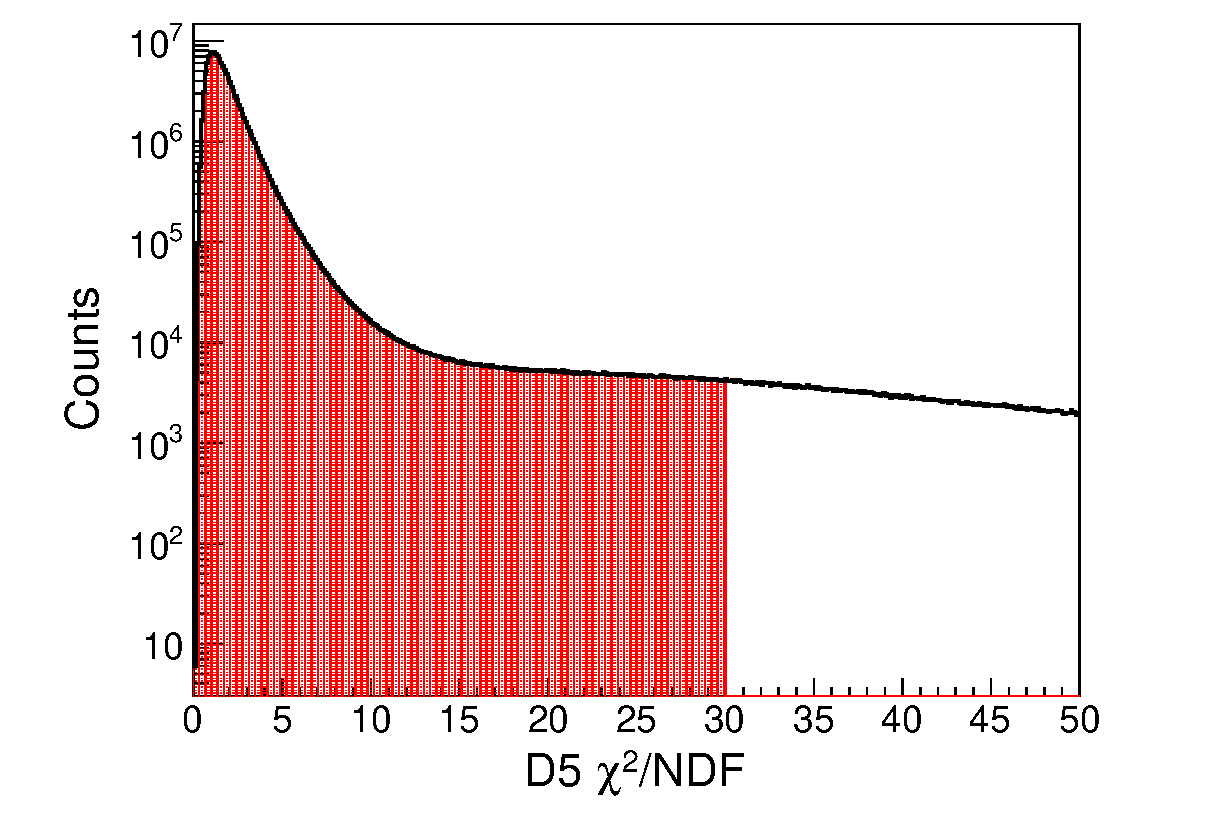
\includegraphics[width=8cm]{../pic/Run78/BL/D5_chi2.eps}
  \caption{
    This figure shows the connected trajectory of BLC1 and BLC2 using the D5 transfer matrix.
    The red hatched region represents an acceptable region.
  }
  \label{fig:D5_chi2}
\end{figure}

\subsection{Beam Momentum Analysis}
\begin{figure}[htbp]
  \centering
  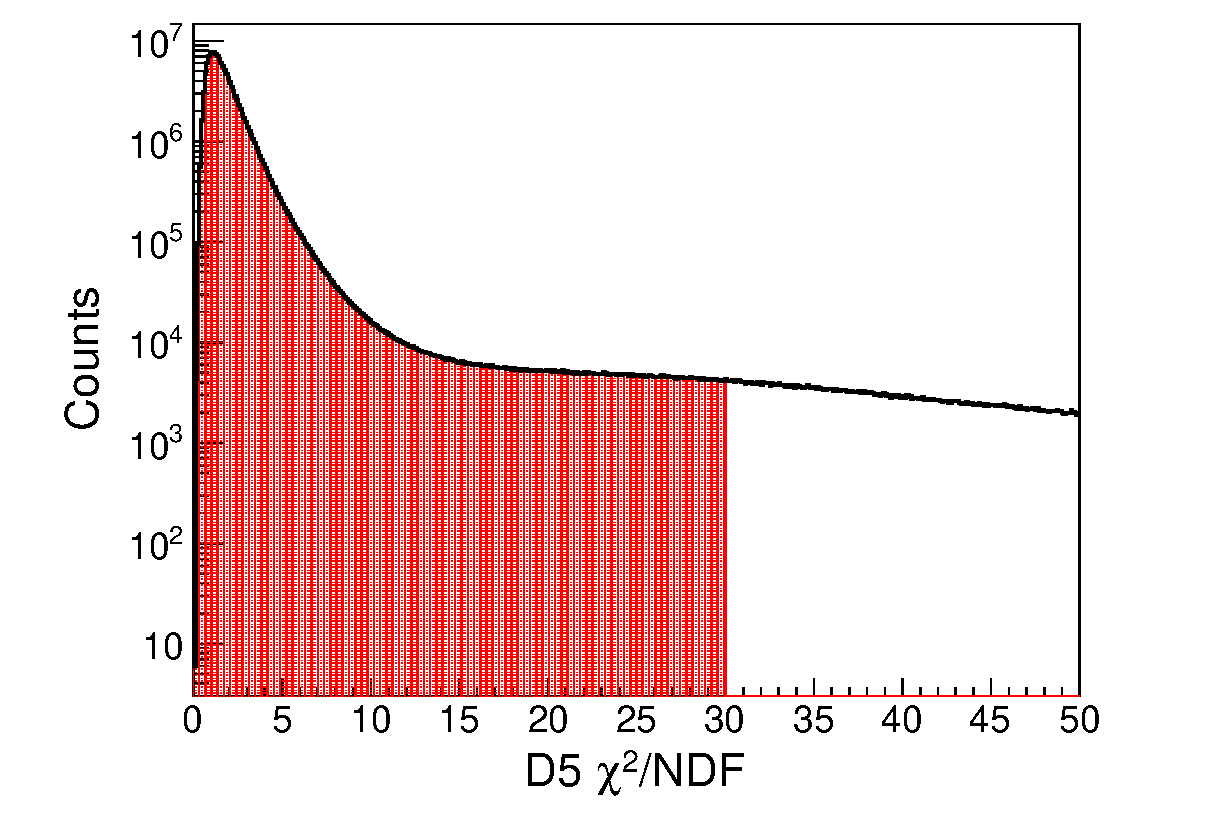
\includegraphics[width=8cm]{../pic/Run78/BL/D5_chi2.eps}
  \caption{
    This figure shows the connected trajectory of BLC1 and BLC2 using the D5 transfer matrix.
    The red hatched region represents an acceptable region.
  }
  \label{fig:D5_chi2}
\end{figure}

\subsection{Beam Momentum Analysis}
\begin{figure}[htbp]
  \centering
  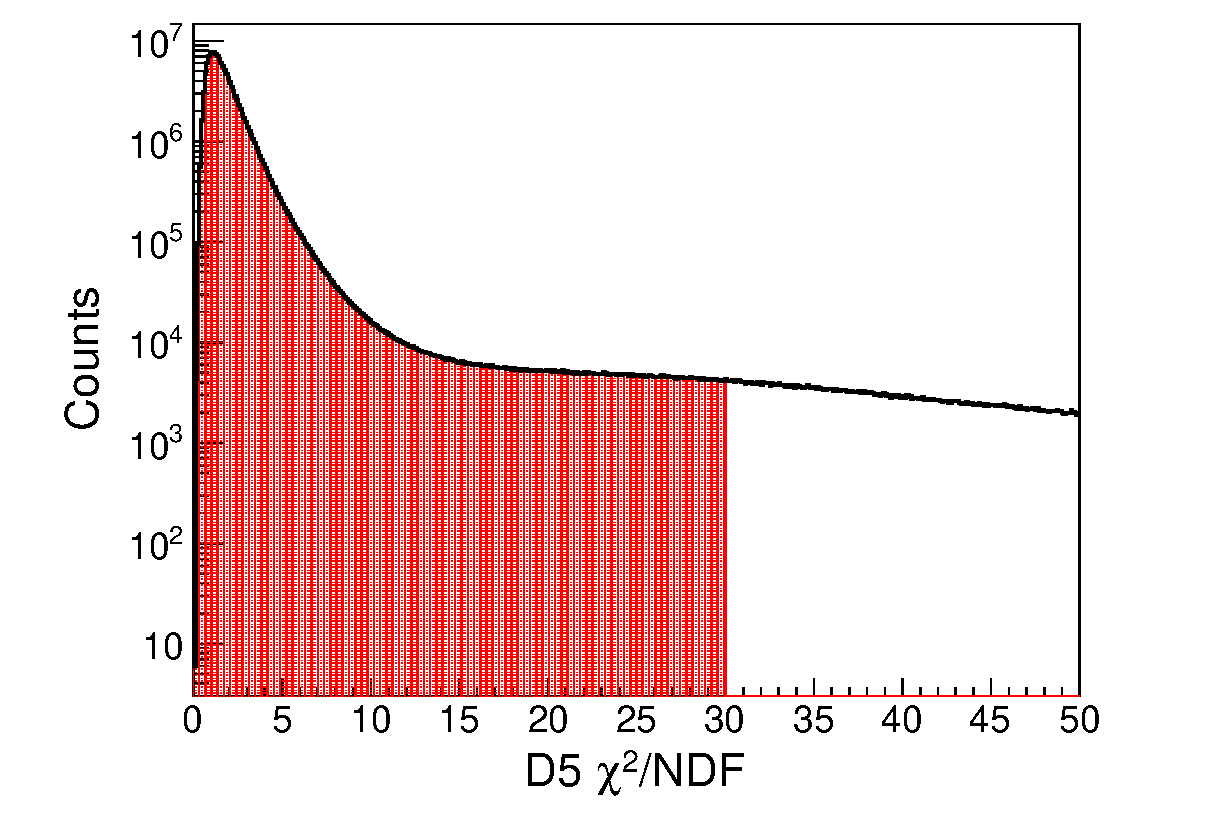
\includegraphics[width=8cm]{../pic/Run78/BL/D5_chi2.eps}
  \caption{
    This figure shows the connected trajectory of BLC1 and BLC2 using the D5 transfer matrix.
    The red hatched region represents an acceptable region.
  }
  \label{fig:D5_chi2}
\end{figure}

\subsection{Beam Momentum Analysis}
\input{analysis/figs/D5_chi}
\input{analysis/figs/beam_mom}
The momentum of the beam is carried out by the D5 magnet and the BLC1 and BLC2 installed upstream and downstream of it.
The beam momentum is measured by connecting the tracks by BLC1 and BLC2 with a second-order transport matrix.
The connection define the $chi^2/NDF$ as shown in Fig.\ref{fig:D5_chi2},
and the $\chi^2/NDF<30$ events are defined as acceptable events.
The left figure in Fig.\ref{fig:beam_mom} shows the measured beam momentum, with the momentum for a BHD of 1 hit also shown as a coloured line.
The BHD is where the beam is widest and there is a correlation between the beam momentum and the BHD segment as shown in the right figurein Fig.\ref{fig:beam_mom}.
Therefore, an acceptance condition is imposed that there is a BHD hit within $3\sigma$ of the analysed beam momentum.

The momentum of the beam is carried out by the D5 magnet and the BLC1 and BLC2 installed upstream and downstream of it.
The beam momentum is measured by connecting the tracks by BLC1 and BLC2 with a second-order transport matrix.
The connection define the $chi^2/NDF$ as shown in Fig.\ref{fig:D5_chi2},
and the $\chi^2/NDF<30$ events are defined as acceptable events.
The left figure in Fig.\ref{fig:beam_mom} shows the measured beam momentum, with the momentum for a BHD of 1 hit also shown as a coloured line.
The BHD is where the beam is widest and there is a correlation between the beam momentum and the BHD segment as shown in the right figurein Fig.\ref{fig:beam_mom}.
Therefore, an acceptance condition is imposed that there is a BHD hit within $3\sigma$ of the analysed beam momentum.

The momentum of the beam is carried out by the D5 magnet and the BLC1 and BLC2 installed upstream and downstream of it.
The beam momentum is measured by connecting the tracks by BLC1 and BLC2 with a second-order transport matrix.
The connection define the $chi^2/NDF$ as shown in Fig.\ref{fig:D5_chi2},
and the $\chi^2/NDF<30$ events are defined as acceptable events.
The left figure in Fig.\ref{fig:beam_mom} shows the measured beam momentum, with the momentum for a BHD of 1 hit also shown as a coloured line.
The BHD is where the beam is widest and there is a correlation between the beam momentum and the BHD segment as shown in the right figurein Fig.\ref{fig:beam_mom}.
Therefore, an acceptance condition is imposed that there is a BHD hit within $3\sigma$ of the analysed beam momentum.

The momentum of the beam is carried out by the D5 magnet and the BLC1 and BLC2 installed upstream and downstream of it.
The beam momentum is measured by connecting the tracks by BLC1 and BLC2 with a second-order transport matrix.
The connection define the $chi^2/NDF$ as shown in Fig.\ref{fig:D5_chi2},
and the $\chi^2/NDF<30$ events are defined as acceptable events.
The left figure in Fig.\ref{fig:beam_mom} shows the measured beam momentum, with the momentum for a BHD of 1 hit also shown as a coloured line.
The BHD is where the beam is widest and there is a correlation between the beam momentum and the BHD segment as shown in the right figurein Fig.\ref{fig:beam_mom}.
Therefore, an acceptance condition is imposed that there is a BHD hit within $3\sigma$ of the analysed beam momentum.
